\subsection{Physics of the interactions}

\begin{description}
\item [Thomson scattering :] During a Thomson scattering, a photon makes
oscillate a free electron. By oscillating, the electron emits a photon at the
same frequency as the incident one. Therefore, the photon is redirected
without any transfer of energy to the medium. Thomson scattering is the
low-energy limit of Compton scattering when the energy of the incident photon
approaches zeros \cite{radiation}.
\item [Rayleigh scattering :] Rayleigh scattering is due to the coherent
action of an atom as a whole. The energy lost by the photon is negligible
\cite{radiation}. The atom recoils because of the momentum conservation. The
Rayleigh scattering is sharply at $0^{\circ}$, especially at low $Z$ and high
energy. The cross section increases as $Z^2$ and decreases with increasing
energy approximately as $h\nu^{-k}$, where $k$ is around 3, $h$ is the
Planck's constant and $\nu$ is the frequency of the radiation \cite{shielding}.
Rayleigh scattering deflects photons from a very well-collimated beam but has
little effect on a broad-beam.
\item [Photoelectric effect :] When a photon undergoes a photoelectric
effect, it is absorbed by an atom which ejects a photoelectron from one of the
bounds shells. The photoelectron appears with a kinetic energy given by :
\begin{equation}
T = h\nu -E_b
\end{equation}
where $E_b$ represents the binding energy of the photoelectron in its original
shell.
The interaction leaves an ionized atom with a vacancy in one
of its bound shells. This hole is quickly filled through the rearrangement of
electrons from other shells of the atom. Therefore, one or more X-ray photons
may also be generated. In some fraction of the cases, the emission of Auger
electrons may substitute for the X-ray. 
\begin{figure}[H]
\centering
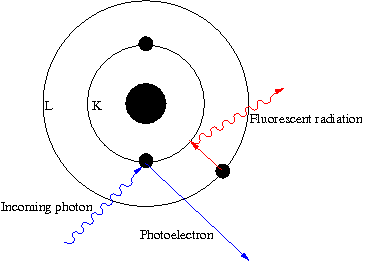
\includegraphics[width=0.5\linewidth]{./Cross_Sections/images/photoelectric}
\caption{Photoelectric effect}
\end{figure}
The photoelectric process is the
predominant mode of interaction for photons of relatively low energy. The
process is more important for high atomic number $Z$. The probability of
photoelectric absorption $\tau$ depends on $Z$ and $h\nu$ as :
\begin{equation}
\tau \propto \frac{Z^n}{\(h\nu\)^3}
\end{equation}
where $n$ varies between 4 and 5. The photoelectric interaction is most likely
to occur if the energy of the incident photon is just greater than the binding
energy of the electron with which it interacts. For photons
of sufficient energy, the most probable origin of the photoelectron is the $K$
shell of the atom \cite{radiation}.
\item [Fluorescence :] Fluorescence is a process in which some of the energy
of a photon is used to create a second photon of different energy. In most
cases, the emitted photon has a longer wavelength, and therefore lower energy,
than the absorbed radiation. However, when two photons are absorbed at the
same time, the emitted photon can have a shorter than the absorbed photons.
\item [Compton effect :] In a Compton interaction, an incident photon loses a
portion of its energy to a free electron and a photon with reduced energy is
produced. The scattered photon leaves the site of the interaction in a
direction from the one of the incident photon. If a photon of energy $h\nu$ 
and momentum $\frac{h\nu}{c}$ ($c$ is the speed of light in vacuum) is  incident 
on a stationary, free electron, after the collision, the photon is scattered at an 
angle $\theta$ with energy $h\nu'$.
\begin{figure}[H]
\centering
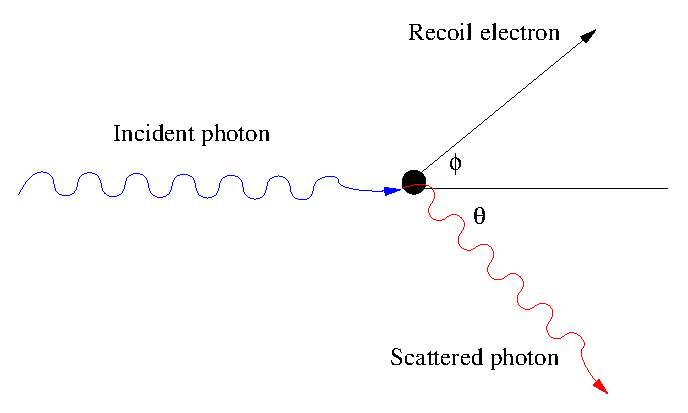
\includegraphics[width=0.5\linewidth]{./Cross_Sections/images/compton}
\caption{Compton effect}
\end{figure}
The Compton shift, i.e. the shift of the wavelength of the photon, is given by :
\begin{equation}
\Delta \lambda = \lambda'-\lambda = \frac{h}{m_e c} \(1-\cos \theta\)
\end{equation}
The Klein-Nishina formal gives the differential cross section of photons
scattered from a single free electron :
\begin{equation}
\frac{d \sigma}{d\bo} = \frac{k_0^2 e^4}{2 m_e^2
c^4}\(\frac{\nu'}{\nu}\)^2\(\frac{\nu}{\nu'}+\frac{\nu'}{\nu}-\sin^2 \theta\)
\end{equation}
where :
\begin{itemize}
\item $\frac{d\sigma}{d\bo}$ is the differential scattering cross sections. It
is the probability per unit solid angle in steradians that a photon, passing
normally through a layer of material containing one electron $m^{-2}$, will be
scattered into a solid $d\bo$ at angle $\theta$.
\item $k_0 = \frac{1}{4\pi \epsilon_0}$, $\epsilon_0$ is the vacuum permittivity
\item $e$ is the elementary charge
\item $m_e$ is the mass of an electron \cite{radiation}
\end{itemize}
\item [Auger electron :] An Auger electron can appear when an $L$ 
electron makes a transition to fill a vacancy in the $K$ shell of an atom. 
Sometimes no photon is emitted and an other $L$ electron can be ejected 
from the atom. The ejected electron is called an Auger electron.
Auger-electron emission is favored over photon emission for elements of low
atomic number. The original inner-shell vacancy can be created by orbital 
electron capture, internal conversion, or
photoelectric effect. Auger cascades can occur in relatively heavy atoms, as
inner-shell vacancies are successively filled by the Auger process, with
simultaneous ejections of the more loosely bound atomic electrons.
\cite{radiation}.
\item [Bremsstrahlung :] Bremsstrahlung is an electromagnetic radiation 
produced by a slowing down or a deflection of charged particle passing through
the electric fields of atomic nuclei. The efficiency of bremsstrahlung varies 
nearly as $Z^2$ 
\cite{radiation}.
\item [Pair production :] During a pair production interaction, an incident
photon interacts with the nuclear Coulomb field (interaction with the Coulomb
field of electron are possible but require more energy) disappears while
producing an electron-positron pair. The momentum is conserved by the nuclear 
recoil. The photon energy appears as the total energy (kinetic plus rest energy) 
of the pair :
\begin{equation}
h\nu = \(E^- + m_e c^2\)+ \(E^+ + m_e c^2\)
\end{equation}
where $E^-$ is the kinetic energy of the electron and $E^+$ is the kinetic
energy of the positron.\\
Given the previous formula, it is obvious that the photon must have an energy 
of at least $2m_e c^2$ to create the electron and positron, hence the threshold 
for pair production is $1.022MeV$. The
kinetic energy $h\nu - 2 m_e c^2$ is distributed between the electron and the
positron. The energy spectra are almost identical and are seldom important
because the interactions of electrons and positrons are almost the same and
their ranges is small. The principal difference is that the positron, after
slowing down, will interact with an electron and releases two $511keV$
annihilation photons, isotropically and back-to-back.\\
The cross section for pair production increases with energy above the
threshold, roughly as $(h\nu)^n$, where $n$ varies from one to two. The cross
sections is proportional to $Z^2$ except above $5MeV$, where the cross section
increases less rapidly because the pair is created further away from the
nucleus and the inner atomic electron form a screen between the nucleus and
the photon\cite{shielding}.
\item [Stopping power :] The stopping power $-\frac{dE}{dx}$ is the energy
loss per unit distance of travel by a charged particle. During the slowing
down, the stopping power generally increases until the energy of the particle is so
low that charge neutralization or quantum effects reduce it. The reason why
the stopping power decrease with increasing energy is called density effect.
The passage of a charged particle through a medium results in
the polarization of the medium. The polarization decreases the electromagnetic 
field acting on the particle reducing the stopping power. This reduction is 
particularly strong in dense media, and is, therefore, called the density effect. 
The density effect increases with particle velocity because distant collisions
become more important at high energies due to Lorentz space contraction. At
very high energies, the density-effect correction is important even in gases
\cite{icru}.\\
\item [Collisional stopping power :] The collision stopping power is due to
energy transfers from the incident particle to bound atomic electrons
\cite{icru}.
The collisional stopping power for
electrons and positrons can be \hbox{written \cite{radiation} :}
\begin{equation}
\(-\frac{dE}{dx}\)_{col}^{\pm} = \frac{4\pi k_0^2 e^4 n}{m_e c^2 \beta^2}
\[\ln \(\frac{m_e c^2 \tau \sqrt{\tau+2}}{\sqrt{2}I}\)+F^{\pm}\(\beta\)\]
\end{equation}
where :
\begin{equation}
F^-(\beta) = \frac{1-\beta^2}{2} \[1+\frac{\tau^2}{8} - (2\tau +1 )\ln 2\]
\end{equation}
is used for electrons and :
\begin{equation}
F^+\(\beta\) = \ln 2 - \frac{\beta^2}{24} \[23 + \frac{14}{\tau +2} +
\frac{10}{\(\tau + 2\)^2} + \frac{4}{\(\tau + 2\)^2}\]
\end{equation}       
for positrons. Here $n$ is number of electrons per unit volume in the medium,
$\beta = \frac{v}{c}$ is the speed of the particle relative to $c$, $I$ is the
mean excitation energy of the medium and $\tau = \frac{T}{m_e c^2}$ is the
kinetic energy $T$ of the particle expressed in multiples of the electron rest
energy $m_ec^2$.\\
The positron-electron differences arises because of the use of the
Bhabha cross section for the positron instead of the M\o ller cross section
for the electron for large energy transfers, and because an electron cannot
loses more than half its entire energy in a single collision, whereas a 
positron can lose its entire energy \cite{icru}.
%A key parameter in the Bethe stopping power is the mean excitation energy of
%the medium. Only moderate accuracy of the mean excitation energy is required
%for the determination of the electron collision stopping power. Let $\Delta 
%S_{col}$ be the uncertainty of $S_{col}$ corresponding to an uncertainty
%$\Delta I$ of $I$. From :
%\begin{equation}
%\frac{S_{col}}{\rho} = \frac{2\pi r_e^2 m c^2}{u} \frac{1}{\beta^2}
%\frac{Z}{A} \[\ln \(\frac{T}{I}\)^2 + \ln\(1+\frac{\tau}{2} + F^-(\tau) -
%\delta \)\]
%\label{supra}
%\end{equation}
%($u$ is the atomic mass unit) where :
%\begin{equation}
%F^-(\tau) = (1-\beta^2)\[ 1+ \frac{\tau^2}{8} - (2\tau+1)\ln 2\]
%\end{equation}
%it can be seen that at low energies, where the density-effect corrections is
%negligible, $\frac{\Delta S_{col}}{S_{col}} = - \frac{(\Delta I/I)}{L}$, where
%the stopping number, $L$, ranges in value from about 3 at 10 keV to about 15
%at 1,000 MeV. At high energies, the $I$-dependence of the density-effect
%correction is such as to reduce the $I$-dependence of the collision stopping
%further; in fact, in the limit of extremely high energies, the collision
%stopping power becomes independent of $I$ \cite{icru}.\\
\item[Radiative stopping power :] The radiative stopping power is due to the
bremsstrahlung. When the energy of the electron is high, the radiation is
emitted mostly in the direction of travel of the electron. Unlike collisional 
energy losses, no single
analytic formula exists for calculating the radiative stopping power. At high
energies bremsstrahlung becomes the predominant mechanism of energy loss for
electrons. The following approximate formula gives the ratio of radiative
and collisional stopping powers for an electron of total energy $E$ (rest +
kinetic energy), expressed
in $MeV$, in an element of atomic number \hbox{$Z$ :}
\begin{equation}
\frac{\(\frac{dE}{dx}\)_{rad}^-}{\(\frac{dE}{dx}\)_{col}^-} \approx
\frac{ZE}{800}
\end{equation}
At very high energies the dominance of radiative over collisional energy
losses gives rise to electron-photon cascade showers. Since bremsstrahlung
photon spectrum is approximately flat out to its maximum (equal to the
electron's kinetic energy), high-energy beta particles emit high-energy
photons. These, in turn, produce Compton electrons and electron-positron
pairs, which then produce additional bremsstrahlung photons, and so on. These
repeated interactions result in an electron-photon cascade shower, which can
be initiated by either a high-energy beta particle or a photon
\cite{radiation}.
\end{description}

